\documentclass[11pt]{article}
\usepackage[a4paper,margin=1in]{geometry}
\usepackage{amsmath,amssymb}
\usepackage{enumitem}
\usepackage{fancyhdr}
\usepackage{array}
\usepackage{needspace}
\usepackage{tikz}

\pagestyle{fancy}
\fancyhf{}
\lhead{\textit{GATE ECE 2027 --- Partial Differential Equations: Notes, Examples, Practice}}
\rhead{\thepage}
\renewcommand{\headrulewidth}{0.6pt}
\setlength{\parindent}{0pt}
\setlength{\parskip}{4pt}
\setlist{itemsep=2pt,topsep=3pt}

\newcommand{\sect}[1]{\Needspace{8\baselineskip}\vspace{1.1em}{\Large\textbf{#1}}\par\vspace{-0.3em}\rule{\textwidth}{0.8pt}\par\vspace{0.2em}}
\newcommand{\key}[1]{\begin{center}\fbox{\parbox{0.93\textwidth}{#1}}\end{center}}
\newcommand{\ex}[1]{\Needspace{7\baselineskip}\vspace{0.9em}\par\noindent\textbf{Example #1.}\ }
\newcommand{\sol}{\par\vspace{2pt}\noindent\textit{Solution.}\ }
\newcommand{\chk}{\par\noindent\textit{Check.}\ }
\newcommand{\warn}[1]{\par\noindent\textit{Watch out:} #1}
\newcommand{\pr}[1]{\Needspace{4\baselineskip}\par\noindent\textbf{#1}\ }

\begin{document}

\begin{center}
{\LARGE \textbf{Partial Differential Equations}}\\[0.5em]
{\large \textit{Concise notes, worked examples and essential practice problems}}\\[0.3em]
{\large \textit{Syllabus: partial differential equations, variable separable method, initial and boundary value problems}}
\end{center}
\rule{\textwidth}{0.8pt}

\textbf{How to use this.} Part 1 is the whole theory you need, in about four pages. Part 2 gives 13 worked examples, each ending with a check. Part 3 has the practice problems, with the essential ones marked $\star$. Part 4 has the answers. You should not need a textbook; a short pointer to Kreyszig is at the end of Part 1 for cross-checking.

\vspace{0.3em}
\textbf{What GATE actually asks.} The usual questions are:
\begin{itemize}
  \item classify a second-order PDE as elliptic, parabolic or hyperbolic;
  \item solve a simple PDE by separation of variables for given conditions, often a first-order one like $u_x=4u_y$;
  \item find the steady-state (long-time) solution of a heat problem;
  \item find eigenvalues and eigenfunctions for given boundary conditions;
  \item recognise the form of the solution of the heat, wave or Laplace equation.
\end{itemize}
\textbf{Not needed:} Fourier or Laplace transform methods for PDEs, Bessel or Legendre functions (circular membranes, spheres), Green's functions, and nonlinear PDEs.

% ============================================================
\newpage
\sect{Part 1: Notes}

\subsection*{1.1\quad Basics and classification}

A PDE has an unknown $u$ of two or more variables. Its \emph{order} is the highest derivative. It is \emph{linear} if $u$ and its derivatives appear only to the first power and are not multiplied together, and \emph{homogeneous} if every term contains $u$. For a linear homogeneous PDE with homogeneous boundary conditions, \textbf{superposition} holds: sums and constant multiples of solutions are solutions. All of separation of variables rests on this.

For a second-order linear PDE $A\,u_{xx}+B\,u_{xy}+C\,u_{yy}+\dots=0$, the sign of the discriminant decides the type:

\begin{center}
\renewcommand{\arraystretch}{1.4}
\begin{tabular}{|l|l|l|}
\hline
\textbf{$B^2-4AC$} & \textbf{Type} & \textbf{Standard example}\\
\hline
$<0$ & Elliptic & Laplace: $u_{xx}+u_{yy}=0$\\
$=0$ & Parabolic & Heat: $u_t=c^2u_{xx}$\\
$>0$ & Hyperbolic & Wave: $u_{tt}=c^2u_{xx}$\\
\hline
\end{tabular}
\end{center}

\subsection*{1.2\quad Initial and boundary conditions}

\begin{itemize}
  \item \textbf{Initial conditions} (IC) are given at $t=0$: the heat equation needs $u(x,0)$; the wave equation needs both $u(x,0)$ and $u_t(x,0)$.
  \item \textbf{Boundary conditions} (BC) are given at the ends. \emph{Dirichlet:} $u=0$ (value fixed). \emph{Neumann:} $u_x=0$ (insulated, no flux). \emph{Mixed:} one of each.
  \item A problem with both is an \emph{initial--boundary value problem}. Laplace's equation has no time, so it needs only boundary conditions (a \emph{boundary value problem}).
\end{itemize}

\subsection*{1.3\quad Separation of variables: the recipe}

Use it for a linear homogeneous PDE with \emph{homogeneous} BCs.

\begin{enumerate}
  \item Assume $u(x,t)=X(x)\,T(t)$ and substitute.
  \item Separate: all $x$ on one side, all $t$ on the other. Both sides must then equal a constant, written $-\lambda$.
  \item Solve the \textbf{spatial eigenvalue problem} $X''+\lambda X=0$ with the BCs. Only special values $\lambda_n$ give non-trivial solutions $X_n$ (table below).
  \item Solve the time equation for each $\lambda_n$.
  \item Superpose: $u=\sum_n X_nT_n$.
  \item Apply the IC to find the constants. This is a Fourier series problem.
\end{enumerate}

\textbf{Why the constant is $-\lambda$ with $\lambda>0$.} For Dirichlet, Neumann or mixed BCs, $\lambda<0$ gives $\cosh,\sinh$ solutions that cannot satisfy the BCs, and $\lambda=0$ gives a straight line that only satisfies them in the Neumann case (a constant). So only $\lambda>0$ (plus $\lambda=0$ for Neumann) survives.

\subsection*{1.4\quad The eigenvalue table (learn this)}

For $X''+\lambda X=0$ on $0<x<L$:

\begin{center}
\renewcommand{\arraystretch}{1.5}
\begin{tabular}{|l|l|l|l|}
\hline
\textbf{Boundary conditions} & \textbf{$\lambda_n$} & \textbf{$X_n(x)$} & \textbf{$n$}\\
\hline
$X(0)=0,\ X(L)=0$ & $\Big(\dfrac{n\pi}{L}\Big)^2$ & $\sin\dfrac{n\pi x}{L}$ & $1,2,3,\dots$\\
$X'(0)=0,\ X'(L)=0$ & $\Big(\dfrac{n\pi}{L}\Big)^2$ & $\cos\dfrac{n\pi x}{L}$ & $0,1,2,\dots$ ($n=0$: constant)\\
$X(0)=0,\ X'(L)=0$ & $\Big(\dfrac{(2n-1)\pi}{2L}\Big)^2$ & $\sin\dfrac{(2n-1)\pi x}{2L}$ & $1,2,3,\dots$\\
$X'(0)=0,\ X(L)=0$ & $\Big(\dfrac{(2n-1)\pi}{2L}\Big)^2$ & $\cos\dfrac{(2n-1)\pi x}{2L}$ & $1,2,3,\dots$\\
\hline
\end{tabular}
\end{center}

\subsection*{1.5\quad The three standard problems (fixed ends, $0<x<L$)}

\key{\textbf{Heat} $u_t=c^2u_{xx}$, $\;u(0,t)=u(L,t)=0$, $\;u(x,0)=f(x)$:
\[
u=\sum_{n\ge1}b_n\,e^{-c^2(n\pi/L)^2t}\sin\frac{n\pi x}{L},\qquad b_n=\frac2L\int_0^Lf(x)\sin\frac{n\pi x}{L}\,dx .
\]
\textbf{Wave} $u_{tt}=c^2u_{xx}$, $\;u(0,t)=u(L,t)=0$, $\;u(x,0)=f(x)$, $\;u_t(x,0)=g(x)$:
\[
u=\sum_{n\ge1}\Big[A_n\cos\frac{n\pi ct}{L}+B_n\sin\frac{n\pi ct}{L}\Big]\sin\frac{n\pi x}{L},
\]
\[
A_n=\frac2L\int_0^Lf\sin\frac{n\pi x}{L}\,dx,\qquad B_n=\frac{2}{n\pi c}\int_0^Lg\sin\frac{n\pi x}{L}\,dx .
\]
\textbf{Laplace} $u_{xx}+u_{yy}=0$ on $0<x<a$, $0<y<b$, with $u=0$ on $x=0$, $x=a$, $y=0$ and $u(x,b)=f(x)$:
\[
u=\sum_{n\ge1}b_n\,\frac{\sinh(n\pi y/a)}{\sinh(n\pi b/a)}\sin\frac{n\pi x}{a},\qquad b_n=\frac2a\int_0^af\sin\frac{n\pi x}{a}\,dx .
\]}

\begin{center}
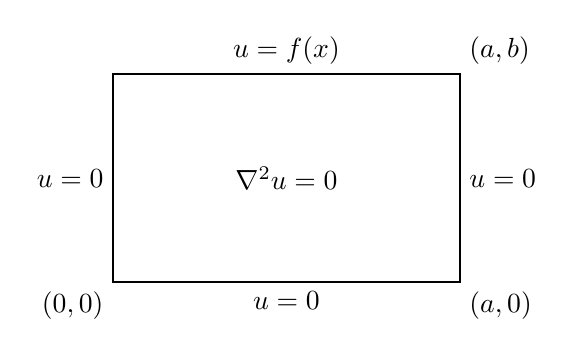
\begin{tikzpicture}[scale=1.1]
\draw[thick] (0,0) rectangle (4,2.4);
\node[below] at (2,0) {$u=0$};
\node[left] at (0,1.2) {$u=0$};
\node[right] at (4,1.2) {$u=0$};
\node[above] at (2,2.4) {$u=f(x)$};
\node[below left] at (0,0) {$(0,0)$};
\node[below right] at (4,0) {$(a,0)$};
\node at (2,1.2) {$\nabla^2u=0$};
\node[above right] at (4,2.4) {$(a,b)$};
\end{tikzpicture}
\end{center}

\textbf{What the formulas say.}
\begin{itemize}
  \item \emph{Heat:} each mode decays at rate $c^2(n\pi/L)^2$, so higher modes die faster. The slowest mode ($n=1$) sets the time constant $\tau=\dfrac{L^2}{c^2\pi^2}$.
  \item \emph{Wave:} modes oscillate with no decay, at angular frequency $\omega_n=n\pi c/L$. The fundamental frequency is $f_1=\dfrac{c}{2L}$ and the motion repeats every $\dfrac{2L}{c}$.
  \item \emph{Laplace:} $\sinh$ in the direction with the non-zero boundary data, $\sin$ along the side where the data is zero at both ends.
  \item \emph{Neumann ends:} use cosines, and include the $n=0$ constant term (the mean of the initial data).
\end{itemize}

\subsection*{1.6\quad Non-homogeneous boundary conditions}

If the heat equation has $u(0,t)=T_1$ and $u(L,t)=T_2$, the separation recipe does not apply directly. Subtract the \textbf{steady state}
\[
u_s(x)=T_1+(T_2-T_1)\frac xL ,
\]
which satisfies the PDE and the BCs. Then $v=u-u_s$ solves the same PDE with \emph{zero} BCs and initial data $v(x,0)=f(x)-u_s(x)$. Solve for $v$ and add $u_s$ back. As $t\to\infty$, $u\to u_s$.

For insulated ends ($u_x=0$ at both), $u\to\dfrac1L\displaystyle\int_0^Lf\,dx$, the average of the initial data.

\subsection*{1.7\quad Fourier coefficients without integrating}

\begin{itemize}
  \item If the IC is already a sum of sines (or cosines) of the right form, \textbf{match coefficients}. No integral is needed.
  \item Otherwise use the standard sine series on $(0,\pi)$ (for general $L$ replace $x$ by $\pi x/L$):
\end{itemize}

\begin{center}
\renewcommand{\arraystretch}{1.5}
\begin{tabular}{|l|l|}
\hline
\textbf{$f(x)$ on $(0,\pi)$} & \textbf{Sine series $\sum b_n\sin nx$}\\
\hline
$1$ & $b_n=\dfrac{4}{n\pi}$ for odd $n$, $0$ for even $n$\\
$x$ & $b_n=\dfrac{2(-1)^{n+1}}{n}$\\
$\pi-x$ & $b_n=\dfrac2n$\\
$x(\pi-x)$ & $b_n=\dfrac{8}{\pi n^3}$ for odd $n$, $0$ for even $n$\\
triangle (peak at $\pi/2$) & $b_n=\dfrac{4}{\pi n^2}\sin\dfrac{n\pi}{2}$ (so odd $n$ only)\\
\hline
\end{tabular}
\end{center}

and one cosine series, $f(x)=x$ on $(0,\pi)$: $\;x=\dfrac\pi2-\dfrac4\pi\displaystyle\sum_{n\ \mathrm{odd}}\dfrac{\cos nx}{n^2}$.

\subsection*{1.8\quad First-order PDEs by separation (very common in GATE)}

For an equation such as $u_x=k\,u_y$ with a condition on one edge, put $u=X(x)Y(y)$. Then $\dfrac{X'}{X}=k\dfrac{Y'}{Y}=\lambda$ (a constant), so $X=e^{\lambda x}$ and $Y=e^{\lambda y/k}$, and $u=Ae^{\lambda(x+y/k)}$. The given condition then fixes $A$ and $\lambda$. Example 2 does this.

\subsection*{1.9\quad Pitfalls}

\begin{itemize}
  \item Check the BCs and IC at the end by substitution. A solution that fails them is wrong however clean it looks.
  \item The wave equation's velocity coefficient is $B_n=\dfrac{2}{n\pi c}\int g\sin(\cdot)$. Forgetting the $\dfrac{1}{n\pi c}$ is the commonest slip.
  \item After subtracting the steady state, the initial data for $v$ is $f-u_s$, not $f$.
  \item Neumann ends have an $n=0$ term; Dirichlet ends do not.
  \item In a first-order separation problem, the sign of the separation constant is decided by the data, not assumed.
\end{itemize}

\key{\textbf{The minimum to memorize.} (i) The discriminant $B^2-4AC$ and its three cases. (ii) The eigenvalue table in 1.4. (iii) The heat and wave solution forms in 1.5. (iv) Subtract the steady state when the BCs are non-zero. (v) The coefficient formula $b_n=\frac2L\int f\sin\frac{n\pi x}{L}$. Everything else can be re-derived with the six-step recipe.}

\textbf{Cross-check in Kreyszig (optional).} Sec.\ 11.1 (p.\ 503) basic concepts, 11.3 (p.\ 507) separation of variables, 11.4 (p.\ 515) d'Alembert, 11.5 (p.\ 520) heat flow, 11.11 (p.\ 547) Laplace's equation. You do not need the other sections of Chapter 11 for this syllabus line.

% ============================================================
\newpage
\sect{Part 2: Worked examples}

\ex{1}
\textbf{(classification)} Classify (a) $u_{xx}+u_{yy}=0$, (b) $u_t=c^2u_{xx}$, (c) $u_{tt}=c^2u_{xx}$, (d) $u_{xx}+2u_{xy}+u_{yy}=0$, (e) $x\,u_{xx}+u_{yy}=0$.
\sol
Read off $A,B,C$ (coefficients of $u_{xx},u_{xy},u_{yy}$, or of the two second derivatives present) and compute $B^2-4AC$.
\begin{itemize}
  \item (a) $A=C=1$, $B=0$: $-4<0$, \textbf{elliptic}.
  \item (b) Only $u_{xx}$ appears: $A=c^2$, $B=C=0$: $0$, \textbf{parabolic}.
  \item (c) Write $-c^2u_{xx}+u_{tt}=0$: $A=-c^2$, $C=1$, $B=0$: $4c^2>0$, \textbf{hyperbolic}.
  \item (d) $A=1$, $B=2$, $C=1$: $4-4=0$, \textbf{parabolic}.
  \item (e) $A=x$, $B=0$, $C=1$: $-4x$. \textbf{Elliptic} for $x>0$, parabolic on $x=0$, \textbf{hyperbolic} for $x<0$. The type can change with position.
\end{itemize}

\ex{2}
\textbf{(first-order PDE by separation)} Solve $u_x=4u_y$ with $u(0,y)=8e^{-3y}$.
\sol
Put $u=X(x)Y(y)$: $X'Y=4XY'$, so $\dfrac{X'}{X}=4\dfrac{Y'}{Y}=k$. Then $X=e^{kx}$ and $Y=e^{ky/4}$, so
\[
u=Ae^{k(x+y/4)}.
\]
At $x=0$: $Ae^{ky/4}=8e^{-3y}$, so $A=8$ and $k/4=-3$, i.e.\ $k=-12$:
\[
\boxed{u=8e^{-12x-3y}}
\]
\chk $u_x=-12u$ and $4u_y=4(-3)u=-12u$ ✓, and $u(0,y)=8e^{-3y}$ ✓.

\ex{3}
\textbf{(an eigenvalue problem)} Find the eigenvalues and eigenfunctions of $X''+\lambda X=0$ with $X(0)=0$, $X'(L)=0$.
\sol
Test each sign of $\lambda$.
\begin{itemize}
  \item $\lambda=0$: $X=ax+b$. $X(0)=0$ gives $b=0$, and $X'(L)=a=0$. Trivial only.
  \item $\lambda=-k^2<0$: $X=A\cosh kx+B\sinh kx$. $X(0)=0$ gives $A=0$. $X'(L)=Bk\cosh kL=0$ forces $B=0$, since $\cosh$ is never zero. Trivial only.
  \item $\lambda=k^2>0$: $X=A\cos kx+B\sin kx$. $X(0)=0$ gives $A=0$. $X'(L)=Bk\cos kL=0$ with $B\neq0$ needs $\cos kL=0$, i.e.\ $kL=\dfrac{(2n-1)\pi}{2}$.
\end{itemize}
\[
\boxed{\lambda_n=\Big(\frac{(2n-1)\pi}{2L}\Big)^2,\qquad X_n=\sin\frac{(2n-1)\pi x}{2L},\qquad n=1,2,\dots}
\]
This is the third row of the table in 1.4.

\ex{4}
\textbf{(heat, sine-sum initial data)} Solve $u_t=4u_{xx}$ on $0<x<\pi$, $u(0,t)=u(\pi,t)=0$, $u(x,0)=2\sin x-\sin3x$.
\sol
Here $c^2=4$, $L=\pi$, so $\lambda_n=n^2$, $X_n=\sin nx$, $T_n=e^{-4n^2t}$. The IC is already a sine sum, so match coefficients: $b_1=2$, $b_3=-1$, others $0$.
\[
\boxed{u=2e^{-4t}\sin x-e^{-36t}\sin3x}
\]
\chk $u_t=-8e^{-4t}\sin x+36e^{-36t}\sin3x$ and $4u_{xx}=-8e^{-4t}\sin x+36e^{-36t}\sin3x$ ✓.

\ex{5}
\textbf{(heat, triangular initial data)} Solve $u_t=u_{xx}$ on $0<x<\pi$, $u(0,t)=u(\pi,t)=0$, with $u(x,0)=x$ for $0\le x\le\pi/2$ and $\pi-x$ for $\pi/2\le x\le\pi$.
\sol
$b_n=\dfrac2\pi\displaystyle\int_0^\pi f\sin nx\,dx$. The triangle is symmetric about $\pi/2$; for odd $n$ the two halves contribute equally and for even $n$ they cancel, so
\[
b_n=\frac4\pi\int_0^{\pi/2}x\sin nx\,dx=\frac4\pi\Big[-\frac{x\cos nx}{n}+\frac{\sin nx}{n^2}\Big]_0^{\pi/2}=\frac{4}{\pi n^2}\sin\frac{n\pi}{2}\quad(n\ \text{odd}),
\]
because $\cos(n\pi/2)=0$ for odd $n$. Since $\sin(n\pi/2)=(-1)^{(n-1)/2}$:
\[
\boxed{u=\frac4\pi\sum_{n\ \mathrm{odd}}\frac{(-1)^{(n-1)/2}}{n^2}\,e^{-n^2t}\sin nx}
\]
\chk At $t=0$, $x=\pi/2$: $\dfrac4\pi\sum_{\mathrm{odd}}\dfrac1{n^2}=\dfrac4\pi\cdot\dfrac{\pi^2}{8}=\dfrac\pi2=f(\pi/2)$ ✓.

\ex{6}
\textbf{(heat, non-homogeneous BCs)} Solve $u_t=u_{xx}$ on $0<x<\pi$, $u(0,t)=0$, $u(\pi,t)=\pi$, $u(x,0)=0$. Find $u$ as $t\to\infty$.
\sol
Steady state: $u_s=T_1+(T_2-T_1)x/L=x$. Put $v=u-x$. Then $v$ has zero BCs and $v(x,0)=-x$.
$b_n=\dfrac2\pi\displaystyle\int_0^\pi(-x)\sin nx\,dx=-\dfrac2\pi\cdot\dfrac{\pi(-1)^{n+1}}{n}=\dfrac{2(-1)^n}{n}$. Hence
\[
\boxed{u=x+2\sum_{n\ge1}\frac{(-1)^n}{n}\,e^{-n^2t}\sin nx}
\]
As $t\to\infty$, $u\to x$ (the steady state).
\chk At $t=0$ the series $2\sum(-1)^n\sin nx/n=-x$, so $u(x,0)=0$ ✓.

\ex{7}
\textbf{(heat, insulated ends)} Solve $u_t=u_{xx}$ on $0<x<\pi$, $u_x(0,t)=u_x(\pi,t)=0$, $u(x,0)=x$.
\sol
Neumann ends give cosines and an $n=0$ term: $u=\dfrac{a_0}{2}+\sum a_n e^{-n^2t}\cos nx$. From the cosine series in 1.7, $a_0=\pi$ and $a_n=-\dfrac{4}{\pi n^2}$ for odd $n$:
\[
\boxed{u=\frac\pi2-\frac4\pi\sum_{n\ \mathrm{odd}}\frac{e^{-n^2t}}{n^2}\cos nx}
\]
As $t\to\infty$, $u\to\pi/2$, the average of the initial temperature, as expected when no heat can escape.

\ex{8}
\textbf{(heat, mixed BCs)} Solve $u_t=u_{xx}$ on $0<x<\pi$, $u(0,t)=0$, $u_x(\pi,t)=0$, $u(x,0)=\sin\frac x2+3\sin\frac{3x}{2}$.
\sol
Mixed BCs (row 3 of the table, $L=\pi$): $\lambda_n=\dfrac{(2n-1)^2}{4}$, $X_n=\sin\dfrac{(2n-1)x}{2}$. The IC matches $n=1$ ($\lambda=\tfrac14$) and $n=2$ ($\lambda=\tfrac94$):
\[
\boxed{u=e^{-t/4}\sin\frac x2+3e^{-9t/4}\sin\frac{3x}{2}}
\]
\chk $u(0,t)=0$; $u_x(\pi,t)=\tfrac12e^{-t/4}\cos\frac\pi2+\tfrac92e^{-9t/4}\cos\frac{3\pi}{2}=0$ ✓.

\ex{9}
\textbf{(wave, plucked string)} A string of length $L$ is fixed at both ends, pulled to height $h$ at the midpoint (triangular shape) and released from rest. Find $u(x,t)$.
\sol
$g=0$, so all $B_n=0$. For a triangle of peak $h$ at $L/2$, $A_n=\dfrac{8h}{n^2\pi^2}\sin\dfrac{n\pi}{2}$ (the table in 1.7 scaled by $h/(L/2)$):
\[
\boxed{u=\frac{8h}{\pi^2}\Big[\cos\frac{\pi ct}{L}\sin\frac{\pi x}{L}-\frac19\cos\frac{3\pi ct}{L}\sin\frac{3\pi x}{L}+\frac1{25}\cos\frac{5\pi ct}{L}\sin\frac{5\pi x}{L}-\cdots\Big]}
\]
Only odd harmonics are present. The fundamental frequency is $c/(2L)$ and the motion repeats every $2L/c$. At $t=L/c$ every odd mode has $\cos n\pi=-1$, so $u(x,L/c)=-f(x)$: the shape is inverted halfway through the period.

\ex{10}
\textbf{(wave, initial velocity)} Solve $u_{tt}=c^2u_{xx}$ on $0<x<\pi$, $u(0,t)=u(\pi,t)=0$, $u(x,0)=0$, $u_t(x,0)=\sin2x$.
\sol
$f=0$ gives $A_n=0$. With $L=\pi$, $u_t(x,0)=\sum B_n\,nc\,\sin nx=\sin2x$, so only $n=2$ survives: $B_2\cdot2c=1$, i.e.\ $B_2=\dfrac1{2c}$.
\[
\boxed{u=\frac{1}{2c}\sin2x\,\sin2ct}
\]
\chk $u_{tt}=-2c\sin2x\sin2ct$ and $c^2u_{xx}=-2c\sin2x\sin2ct$ ✓; $u_t(x,0)=\sin2x$ ✓.

\ex{11}
\textbf{(d'Alembert, infinite string)} Solve $u_{tt}=4u_{xx}$ on $-\infty<x<\infty$ with $u(x,0)=\sin x$ and $u_t(x,0)=x$.
\sol
d'Alembert: $u=\tfrac12\big[f(x+ct)+f(x-ct)\big]+\dfrac{1}{2c}\displaystyle\int_{x-ct}^{x+ct}g(s)\,ds$, with $c=2$:
\[
u=\tfrac12\big[\sin(x+2t)+\sin(x-2t)\big]+\frac14\int_{x-2t}^{x+2t}s\,ds=\sin x\cos2t+\frac14\cdot4xt .
\]
\[
\boxed{u=\sin x\cos2t+xt}
\]
\chk $u_{tt}=-4\sin x\cos2t=4u_{xx}$ ✓; $u(x,0)=\sin x$ ✓; $u_t(x,0)=x$ ✓.

\ex{12}
\textbf{(Laplace in a square, and a symmetry shortcut)} A square plate $0<x,y<\pi$ has the edges $x=0$, $x=\pi$, $y=0$ held at $0$ and the edge $y=\pi$ held at $100$. Find $u$ and the temperature at the centre.
\sol
Use the Laplace formula in 1.5 with $a=b=\pi$ and $f=100$. From the table, $b_n=100\cdot\dfrac{4}{n\pi}=\dfrac{400}{n\pi}$ for odd $n$:
\[
\boxed{u=\frac{400}{\pi}\sum_{n\ \mathrm{odd}}\frac{\sinh ny}{n\sinh n\pi}\,\sin nx}
\]
\emph{Centre by symmetry (no series needed).} Four copies of this problem, with the hot edge in turn on each of the four sides, add up (by superposition) to the plate with all four edges at $100$, whose solution is $u\equiv100$. By symmetry all four have the same centre value, so each gives $\dfrac{100}{4}=\boxed{25}$.
\chk Summing the series at $(\pi/2,\pi/2)$ gives $\dfrac{200}{\pi}\sum_{n\ \mathrm{odd}}\dfrac{(-1)^{(n-1)/2}}{n\cosh(n\pi/2)}\approx63.66\times0.3927=25.0$ ✓.

\ex{13}
\textbf{(time scale of heat flow)} A rod of length $L=1$ m has diffusivity $c^2=10^{-4}$ m$^2$/s and both ends held at $0$. Estimate the time for the slowest mode to fall to $1\%$.
\sol
The slowest mode decays as $e^{-t/\tau}$ with $\tau=\dfrac{L^2}{c^2\pi^2}=\dfrac{1}{10^{-4}\pi^2}\approx1013$ s. Falling to $1\%$ takes $t=\tau\ln100\approx1013\times4.605\approx4.7\times10^3$ s, about $78$ minutes. Since $\tau\propto L^2$, doubling the length makes the decay four times slower.

% ============================================================
\newpage
\sect{Part 3: Practice problems}

Do the problems marked $\star$ first. Answers are in Part 4.

\subsection*{A. Classification and first-order PDEs}
\pr{A1$\star$.} Classify (a) $3u_{xx}+2u_{xy}+u_{yy}=0$, (b) $u_{xx}-4u_{xy}+4u_{yy}=0$, (c) $u_{xx}+5u_{xy}+4u_{yy}=0$, (d) $y\,u_{xx}+u_{yy}=0$.

\pr{A2$\star$.} Solve $u_x=3u_y$ with $u(0,y)=5e^{-6y}$.

\pr{A3$\star$.} Solve $3u_x+2u_y=0$ with $u(x,0)=4e^{-x}$.

\subsection*{B. Eigenvalue problems}
\pr{B1$\star$.} Find the eigenvalues and eigenfunctions of $X''+\lambda X=0$ with $X'(0)=0$, $X(L)=0$.

\pr{B2.} Show that $X''+\lambda X=0$, $X(0)=X(L)=0$ has no non-trivial solution for $\lambda\le0$.

\subsection*{C. Heat equation}
\pr{C1$\star$.} Solve $u_t=u_{xx}$ on $0<x<\pi$, $u(0,t)=u(\pi,t)=0$, $u(x,0)=3\sin2x-\sin5x$.

\pr{C2.} Same equation and BCs with $u(x,0)=1$ (uniform initial temperature).

\pr{C3$\star$.} Solve $u_t=u_{xx}$ on $0<x<1$, $u(0,t)=0$, $u(1,t)=1$, $u(x,0)=0$. What is $\lim_{t\to\infty}u$?

\pr{C4$\star$.} Solve $u_t=u_{xx}$ on $0<x<\pi$, $u_x(0,t)=u_x(\pi,t)=0$, $u(x,0)=\cos^2x$.

\pr{C5$\star$.} Solve $u_t=u_{xx}$ on $0<x<\pi$, $u(0,t)=0$, $u_x(\pi,t)=0$, $u(x,0)=\sin\frac x2-2\sin\frac{5x}{2}$.

\pr{C6.} A rod of length $2$ has its ends held at $10^\circ$ and $50^\circ$. Find the steady-state temperature at $x=0.5$.

\pr{C7.} In a rod with fixed-temperature ends, if the length is doubled and the material is unchanged, by what factor does the slowest decay time change?

\pr{C8.} A rod of length $\pi$ with insulated ends has initial temperature $u(x,0)=x$. What is the limiting temperature as $t\to\infty$?

\subsection*{D. Wave equation}
\pr{D1$\star$.} Solve $u_{tt}=9u_{xx}$ on $0<x<\pi$, $u(0,t)=u(\pi,t)=0$, $u(x,0)=\sin x$, $u_t(x,0)=2\sin4x$.

\pr{D2.} A string of length $L$ fixed at both ends has wave speed $c$. Find its fundamental frequency. If the tension is quadrupled (with $c\propto\sqrt T$), what happens to the fundamental frequency?

\pr{D3$\star$.} Use d'Alembert's formula to solve $u_{tt}=c^2u_{xx}$ with $u(x,0)=x^2$, $u_t(x,0)=2x$.

\pr{D4.} Solve $u_{tt}=c^2u_{xx}$ with $u(x,0)=\cos x$, $u_t(x,0)=0$.

\subsection*{E. Laplace equation}
\pr{E1$\star$.} Solve $u_{xx}+u_{yy}=0$ on $0<x<\pi$, $0<y<\pi$ with $u=0$ on $x=0$, $x=\pi$, $y=0$ and $u(x,\pi)=\sin2x+4\sin5x$.

\pr{E2$\star$.} A square plate has one edge at $100^\circ$ and the other three edges at $0^\circ$. What is the temperature at the centre?

\pr{E3.} A square plate has two \emph{opposite} edges at $100^\circ$ and the other two at $0^\circ$. What is the temperature at the centre?

\pr{E4.} Which of $x^2-y^2$, $x^2+y^2$, $e^x\cos y$, $xy$ satisfy Laplace's equation?

% ============================================================
\newpage
\sect{Part 4: Answers and hints}

\renewcommand{\arraystretch}{1.5}
\begin{longtable}{|p{1.4cm}|p{14cm}|}
\hline
\textbf{No.} & \textbf{Answer and hint}\\
\hline
A1 & $B^2-4AC$: (a) $4-12=-8$, \textbf{elliptic}. (b) $16-16=0$, \textbf{parabolic}. (c) $25-16=9$, \textbf{hyperbolic}. (d) $-4y$: elliptic for $y>0$, parabolic at $y=0$, hyperbolic for $y<0$.\\
\hline
A2 & $u=5e^{-18x-6y}$. Separate: $X'/X=3Y'/Y=k$, $u=Ae^{k(x+y/3)}$; matching $e^{ky/3}=e^{-6y}$ gives $k=-18$.\\
\hline
A3 & $u=4e^{-x+3y/2}$. Separate: $3X'/X=-2Y'/Y=k$, so $X=e^{kx/3}$, $Y=e^{-ky/2}$; matching $e^{kx/3}=e^{-x}$ gives $k=-3$.\\
\hline
B1 & $\lambda_n=\Big(\dfrac{(2n-1)\pi}{2L}\Big)^2$, $X_n=\cos\dfrac{(2n-1)\pi x}{2L}$, $n=1,2,\dots$ (the fourth row of the table; $X'(0)=0$ forces cosine, $X(L)=0$ forces $\cos kL=0$).\\
\hline
B2 & $\lambda=0$: $X=ax+b$, and $X(0)=X(L)=0$ gives $a=b=0$. $\lambda=-k^2$: $X=A\cosh kx+B\sinh kx$, $X(0)=0\Rightarrow A=0$, then $B\sinh kL=0\Rightarrow B=0$ since $\sinh kL\neq0$ for $k>0$.\\
\hline
C1 & $u=3e^{-4t}\sin2x-e^{-25t}\sin5x$. Match coefficients; decay factor $e^{-n^2t}$.\\
\hline
C2 & $u=\dfrac4\pi\displaystyle\sum_{n\ \mathrm{odd}}\dfrac{e^{-n^2t}}{n}\sin nx$ (the coefficients of $f=1$ from the table).\\
\hline
C3 & $u=x+\displaystyle\sum_{n\ge1}\dfrac{2(-1)^n}{n\pi}\,e^{-n^2\pi^2t}\sin n\pi x$, and $u\to x$ as $t\to\infty$. Steady state $u_s=x$; $v=u-x$ has $v(x,0)=-x$.\\
\hline
C4 & $u=\tfrac12+\tfrac12e^{-4t}\cos2x$, since $\cos^2x=\tfrac12+\tfrac12\cos2x$ is already a cosine series ($n=0$ and $n=2$).\\
\hline
C5 & $u=e^{-t/4}\sin\dfrac x2-2e^{-25t/4}\sin\dfrac{5x}{2}$ (mixed BCs: $\lambda=(2n-1)^2/4$; the terms are $n=1$ and $n=3$).\\
\hline
C6 & $20^\circ$. Steady state $u_s=10+20x$.\\
\hline
C7 & Four times slower, since $\tau=L^2/(c^2\pi^2)\propto L^2$.\\
\hline
C8 & $\pi/2$, the average of $f$ over the rod: $\frac1\pi\int_0^\pi x\,dx$.\\
\hline
D1 & $u=\sin x\cos3t+\tfrac16\sin4x\sin12t$. First term from $f$ ($A_1=1$, frequency $nc=3$); second from $g$: $B_4\cdot4c=2$ with $c=3$ gives $B_4=\tfrac16$.\\
\hline
D2 & $f_1=\dfrac{c}{2L}$. Quadrupling the tension doubles $c$, so the fundamental frequency \textbf{doubles}.\\
\hline
D3 & $u=x^2+2xt+c^2t^2$. The first part gives $x^2+c^2t^2$; $\dfrac1{2c}\int_{x-ct}^{x+ct}2s\,ds=2xt$.\\
\hline
D4 & $u=\cos x\,\cos ct$, from $\tfrac12\big[\cos(x+ct)+\cos(x-ct)\big]$.\\
\hline
E1 & $u=\dfrac{\sin2x\,\sinh2y}{\sinh2\pi}+4\dfrac{\sin5x\,\sinh5y}{\sinh5\pi}$. Match coefficients: $b_2=1$, $b_5=4$ on the edge $y=\pi$.\\
\hline
E2 & $25^\circ$, by the symmetry argument in Example 12.\\
\hline
E3 & $50^\circ$. Each hot edge alone gives $25^\circ$ at the centre; add them by superposition.\\
\hline
E4 & $x^2-y^2$, $e^x\cos y$ and $xy$ are harmonic. $x^2+y^2$ is not: its Laplacian is $4$.\\
\hline
\end{longtable}

\end{document}
